\documentclass[11pt,a4paper,]{article}
\usepackage{lmodern}

\usepackage{amssymb,amsmath}
\usepackage{ifxetex,ifluatex}
\usepackage{fixltx2e} % provides \textsubscript
\ifnum 0\ifxetex 1\fi\ifluatex 1\fi=0 % if pdftex
  \usepackage[T1]{fontenc}
  \usepackage[utf8]{inputenc}
\else % if luatex or xelatex
  \usepackage{unicode-math}
  \defaultfontfeatures{Ligatures=TeX,Scale=MatchLowercase}
\fi
% use upquote if available, for straight quotes in verbatim environments
\IfFileExists{upquote.sty}{\usepackage{upquote}}{}
% use microtype if available
\IfFileExists{microtype.sty}{%
\usepackage[]{microtype}
\UseMicrotypeSet[protrusion]{basicmath} % disable protrusion for tt fonts
}{}
\PassOptionsToPackage{hyphens}{url} % url is loaded by hyperref
\usepackage[unicode=true]{hyperref}
\hypersetup{
            pdftitle={Expert advice from experts},
            pdfborder={0 0 0},
            breaklinks=true}
\urlstyle{same}  % don't use monospace font for urls
\usepackage{geometry}
\geometry{a4paper, centering, text={16cm,24cm}}
\usepackage[style=authoryear-comp,]{biblatex}
\addbibresource{references.bib}
\usepackage{longtable,booktabs}
% Fix footnotes in tables (requires footnote package)
\IfFileExists{footnote.sty}{\usepackage{footnote}\makesavenoteenv{long table}}{}
\usepackage{graphicx,grffile}
\makeatletter
\def\maxwidth{\ifdim\Gin@nat@width>\linewidth\linewidth\else\Gin@nat@width\fi}
\def\maxheight{\ifdim\Gin@nat@height>\textheight\textheight\else\Gin@nat@height\fi}
\makeatother
% Scale images if necessary, so that they will not overflow the page
% margins by default, and it is still possible to overwrite the defaults
% using explicit options in \includegraphics[width, height, ...]{}
\setkeys{Gin}{width=\maxwidth,height=\maxheight,keepaspectratio}
\IfFileExists{parskip.sty}{%
\usepackage{parskip}
}{% else
\setlength{\parindent}{0pt}
\setlength{\parskip}{6pt plus 2pt minus 1pt}
}
\setlength{\emergencystretch}{3em}  % prevent overfull lines
\providecommand{\tightlist}{%
  \setlength{\itemsep}{0pt}\setlength{\parskip}{0pt}}
\setcounter{secnumdepth}{5}

% set default figure placement to htbp
\makeatletter
\def\fps@figure{htbp}
\makeatother


\title{Expert advice from experts}

%% MONASH STUFF

%% CAPTIONS
\RequirePackage{caption}
\DeclareCaptionStyle{italic}[justification=centering]
 {labelfont={bf},textfont={it},labelsep=colon}
\captionsetup[figure]{style=italic,format=hang,singlelinecheck=true}
\captionsetup[table]{style=italic,format=hang,singlelinecheck=true}


%% FONT
\RequirePackage{bera}
\RequirePackage[charter,expert,sfscaled]{mathdesign}
\RequirePackage{fontawesome}

%% HEADERS AND FOOTERS
\RequirePackage{fancyhdr}
\pagestyle{fancy}
\rfoot{\Large\sffamily\raisebox{-0.1cm}{\textbf{\thepage}}}
\makeatletter
\lhead{\textsf{\expandafter{\@title}}}
\makeatother
\rhead{}
\cfoot{}
\setlength{\headheight}{15pt}
\renewcommand{\headrulewidth}{0.4pt}
\renewcommand{\footrulewidth}{0.4pt}
\fancypagestyle{plain}{%
\fancyhf{} % clear all header and footer fields
\fancyfoot[C]{\sffamily\thepage} % except the center
\renewcommand{\headrulewidth}{0pt}
\renewcommand{\footrulewidth}{0pt}}

%% MATHS
\RequirePackage{bm,amsmath}
\allowdisplaybreaks

%% GRAPHICS
\RequirePackage{graphicx}
\setcounter{topnumber}{2}
\setcounter{bottomnumber}{2}
\setcounter{totalnumber}{4}
\renewcommand{\topfraction}{0.85}
\renewcommand{\bottomfraction}{0.85}
\renewcommand{\textfraction}{0.15}
\renewcommand{\floatpagefraction}{0.8}


%\RequirePackage[section]{placeins}

%% SECTION TITLES


%% SECTION TITLES
\RequirePackage[compact,sf,bf]{titlesec}
\titleformat*{\section}{\Large\sf\bfseries\color[rgb]{0.7,0,0}}
\titleformat*{\subsection}{\large\sf\bfseries\color[rgb]{0.7,0,0}}
\titleformat*{\subsubsection}{\sf\bfseries\color[rgb]{0.7,0,0}}
\titlespacing{\section}{0pt}{2ex}{.5ex}
\titlespacing{\subsection}{0pt}{1.5ex}{0ex}
\titlespacing{\subsubsection}{0pt}{.5ex}{0ex}


%% TITLE PAGE
\def\Date{\number\day}
\def\Month{\ifcase\month\or
 January\or February\or March\or April\or May\or June\or
 July\or August\or September\or October\or November\or December\fi}
\def\Year{\number\year}

%% LINE AND PAGE BREAKING
\sloppy
\clubpenalty = 10000
\widowpenalty = 10000
\brokenpenalty = 10000
\RequirePackage{microtype}

%% PARAGRAPH BREAKS
\setlength{\parskip}{1.4ex}
\setlength{\parindent}{0em}

%% HYPERLINKS
\RequirePackage{xcolor} % Needed for links
\definecolor{darkblue}{rgb}{0,0,.6}
\RequirePackage{url}

\makeatletter
\@ifpackageloaded{hyperref}{}{\RequirePackage{hyperref}}
\makeatother
\hypersetup{
     citecolor=0 0 0,
     breaklinks=true,
     bookmarksopen=true,
     bookmarksnumbered=true,
     linkcolor=darkblue,
     urlcolor=blue,
     citecolor=darkblue,
     colorlinks=true}

\usepackage[showonlyrefs]{mathtools}
\usepackage[no-weekday]{eukdate}

%% BIBLIOGRAPHY

\makeatletter
\@ifpackageloaded{biblatex}{}{\usepackage[style=authoryear-comp, backend=biber, natbib=true]{biblatex}}
\makeatother
\ExecuteBibliographyOptions{bibencoding=utf8,minnames=1,maxnames=3, maxbibnames=99,dashed=false,terseinits=true,giveninits=true,uniquename=false,uniquelist=false,doi=false, isbn=false,url=true,sortcites=false}

\DeclareFieldFormat{url}{\texttt{\url{#1}}}
\DeclareFieldFormat[article]{pages}{#1}
\DeclareFieldFormat[inproceedings]{pages}{\lowercase{pp.}#1}
\DeclareFieldFormat[incollection]{pages}{\lowercase{pp.}#1}
\DeclareFieldFormat[article]{volume}{\mkbibbold{#1}}
\DeclareFieldFormat[article]{number}{\mkbibparens{#1}}
\DeclareFieldFormat[article]{title}{\MakeCapital{#1}}
\DeclareFieldFormat[article]{url}{}
%\DeclareFieldFormat[book]{url}{}
%\DeclareFieldFormat[inbook]{url}{}
%\DeclareFieldFormat[incollection]{url}{}
%\DeclareFieldFormat[inproceedings]{url}{}
\DeclareFieldFormat[inproceedings]{title}{#1}
\DeclareFieldFormat{shorthandwidth}{#1}
%\DeclareFieldFormat{extrayear}{}
% No dot before number of articles
\usepackage{xpatch}
\xpatchbibmacro{volume+number+eid}{\setunit*{\adddot}}{}{}{}
% Remove In: for an article.
\renewbibmacro{in:}{%
  \ifentrytype{article}{}{%
  \printtext{\bibstring{in}\intitlepunct}}}

\AtEveryBibitem{\clearfield{month}}
\AtEveryCitekey{\clearfield{month}}

\makeatletter
\DeclareDelimFormat[cbx@textcite]{nameyeardelim}{\addspace}
\makeatother

\author{\sf\Large\textbf{ Marie Curie}\\ {\sf\large Nobel Prize, PhD\\[0.5cm]} \sf\Large\textbf{ Pierre Curie}\\ {\sf\large Nobel Prize, PhD\\[0.5cm]}}

\date{\sf\Date~\Month~\Year}
\makeatletter
\lfoot{\sf Curie, Curie: \@date}
\makeatother


%%%% PAGE STYLE FOR FRONT PAGE OF REPORTS

\makeatletter
\def\organization#1{\gdef\@organization{#1}}
\def\telephone#1{\gdef\@telephone{#1}}
\def\email#1{\gdef\@email{#1}}
\makeatother
  \organization{Acme Corporation}

  \def\name{Department of\newline Econometrics \&\newline Business Statistics}

  \telephone{(03) 9905 2478}

  \email{BusEco-Econometrics@monash.edu}

\def\webaddress{\url{http://buseco.monash.edu/ebs/consulting/}}
\def\abn{12 377 614 012}
\def\logo{
\includegraphics[width=6cm]{MBSportrait}}
\def\extraspace{\vspace*{1.6cm}}
\makeatletter
\def\contactdetails{\faicon{phone} & \@telephone \\
                    \faicon{envelope} & \@email}
\makeatother

%%%% FRONT PAGE OF REPORTS

\def\reporttype{Report for}

\long\def\front#1#2#3{
\newpage
\begin{singlespacing}
\thispagestyle{empty}
\vspace*{-1.4cm}
\hspace*{-1.4cm}
\hbox to 16cm{
  \hbox to 6.5cm{\vbox to 14cm{\vbox to 25cm{
    \logo
    \vfill
    \parbox{6.3cm}{\raggedright
      \sf\color[rgb]{0.00,0.00,0.70}
      {\large\textbf{\name}}\par
      \vspace{.7cm}
      \tabcolsep=0.12cm\sf\small
      \begin{tabular}{@{}ll@{}}\contactdetails
      \end{tabular}
      \vspace*{0.3cm}\par
      ABN: \abn\par
    }
  }\vss}\hss}
  \hspace*{0.2cm}
  \hbox to 1cm{\vbox to 14cm{\rule{1pt}{26.8cm}\vss}\hss\hfill}
  \hbox to 10cm{\vbox to 14cm{\vbox to 25cm{
      \vspace*{3cm}\sf\raggedright
      \parbox{11cm}{\sf\raggedright\baselineskip=1.2cm
         \fontsize{24.88}{30}\color[rgb]{0.70,0.00,0.00}\sf\textbf{#1}}
      \par
      \vfill
      \large
      \vbox{\parskip=0.8cm #2}\par
      \vspace*{2cm}\par
      \reporttype\\[0.3cm]
      \hbox{#3}%\\[2cm]\
      \vspace*{1cm}
      {\large\sf\textbf{\Date~\Month~\Year}}
   }\vss}
  }}
\end{singlespacing}
\newpage
}

\makeatletter
\def\titlepage{\front{\expandafter{\@title}}{\@author}{\@organization}}
\makeatother

\usepackage{setspace}
\setstretch{1.5}

%% Any special functions or other packages can be loaded here.


\begin{document}
\titlepage

147 variables with 102 having the missing value

\begin{verbatim}
##      Name              Symbol             Market             Sector         
##  Length:45          Length:45          Length:45          Length:45         
##  Class :character   Class :character   Class :character   Class :character  
##  Mode  :character   Mode  :character   Mode  :character   Mode  :character  
##                                                                             
##                                                                             
##                                                                             
##    Industry           intra_day           ent_value            trail_pe     
##  Length:45          Min.   :      6.4   Min.   :      7.8   Min.   :  7.54  
##  Class :character   1st Qu.:     36.3   1st Qu.:     59.3   1st Qu.: 17.26  
##  Mode  :character   Median :     79.6   Median :    122.4   Median : 24.74  
##                     Mean   :  71455.7   Mean   :  70367.6   Mean   : 46.22  
##                     3rd Qu.:    204.8   3rd Qu.:    241.0   3rd Qu.: 41.50  
##                     Max.   :1670000.0   Max.   :1670000.0   Max.   :769.92  
##      for_pe           peg              ttm             mrq        
##  Min.   : 3.59   Min.   :-27.96   Min.   : 0.25   Min.   : 0.620  
##  1st Qu.:14.62   1st Qu.:  1.34   1st Qu.: 1.17   1st Qu.: 2.490  
##  Median :18.54   Median :  2.39   Median : 3.08   Median : 5.320  
##  Mean   :21.90   Mean   : 19.23   Mean   : 4.40   Mean   : 7.352  
##  3rd Qu.:25.85   3rd Qu.:  4.19   3rd Qu.: 5.94   3rd Qu.:11.710  
##  Max.   :98.25   Max.   :713.67   Max.   :18.62   Max.   :28.070  
##       rev             ebitda         tot_risk       envir_risk    
##  Min.   : 0.560   Min.   : 5.69   Min.   :11.00   Min.   : 0.000  
##  1st Qu.: 1.420   1st Qu.:11.48   1st Qu.:17.00   1st Qu.: 1.000  
##  Median : 3.670   Median :14.68   Median :20.00   Median : 2.000  
##  Mean   : 4.779   Mean   :18.52   Mean   :22.78   Mean   : 4.333  
##  3rd Qu.: 6.940   3rd Qu.:21.38   3rd Qu.:27.00   3rd Qu.: 7.000  
##  Max.   :17.570   Max.   :83.52   Max.   :40.00   Max.   :18.000  
##   social_risk      gover_risk  
##  Min.   : 3.00   Min.   : 4.0  
##  1st Qu.: 7.00   1st Qu.: 6.0  
##  Median :10.00   Median : 7.0  
##  Mean   :10.76   Mean   : 7.6  
##  3rd Qu.:14.00   3rd Qu.: 9.0  
##  Max.   :25.00   Max.   :12.0
\end{verbatim}

\hypertarget{description-of-the-variables-related-to-the-value-of-stocks}{%
\subsection{Description of the variables related to the value of stocks:}\label{description-of-the-variables-related-to-the-value-of-stocks}}

\begin{itemize}
\tightlist
\item
  Market capitalization refers to how much a company is worth as determined by the stock market. It is defined as the total market value of all outstanding shares. To calculate a company's market cap, multiply the number of outstanding shares by the current market value of one share. Companies are typically divided according to market capitalization: large-cap (\$10 billion or more), mid-cap (\$2 billion to \$10 billion), and small-cap (\$300 million to \$2 billion). Enterprise value includes in its calculation the market capitalization of a company but also short-term and long-term debt as well as any cash on the company's balance sheet. Enterprise value is used as the basis for many financial ratios that measure the performance of a company.
\item
  Enterprise value (EV) is a measure of a company's total value, often used as a more comprehensive alternative to equity market capitalization.
\item
  Trailing P/E is calculated by dividing the current market value, or share price, by the earnings per share over the previous 12 months.
\item
  The forward P/E ratio estimates a company's likely earnings per share for the next 12 months.
\item
  The PEG ratio enhances the P/E ratio by adding in expected earnings growth into the calculation. The PEG ratio is considered to be an indicator of a stock's true value, and similar to the P/E ratio, a \emph{lower PEG may indicate that a stock is undervalued}.
\item
  The P/S ratio is a key analysis and valuation tool that shows \emph{how much investors are willing to pay per dollar of sales for a stock.} The P/S ratio is typically calculated by dividing the stock price by the underlying company's sales per share.A low ratio could imply the stock is undervalued while a ratio that is higher-than-average could indicate that the stock is overvalued.
\item
  The P/B ratio measures the market's valuation of a company relative to its book value.\emph{The market value of equity is typically higher than the book value of a company.} P/B ratio is used by value investors to identify potential investments. P/B ratios under 1 are typically considered solid investments.
\item
  The enterprise value-to-revenue (EV/R) multiple helps compares a company's revenues to its enterprise value. \emph{The lower the better, in that, a lower EV/R multiple signals a company is undervalued.}
\item
  The enterprise value to earnings before interest, taxes, depreciation, and amortization ratio (EV/EBITDA) compares the value of a company---debt included---to the company's cash earnings less non-cash expenses. The EV/EBITDA metric is a popular valuation tool that helps investors compare companies in order to make an investment decision. EV calculates a company's total value or assessed worth, while EBITDA measures a company's overall financial performance and profitability. Typically, when evaluating a company, \emph{an EV/EBITDA value below 10 is seen as healthy}. It's best to use the EV/EBITDA metric when comparing companies within the same industry or sector.
\end{itemize}

\hypertarget{value-analysis}{%
\subsection{Value Analysis}\label{value-analysis}}

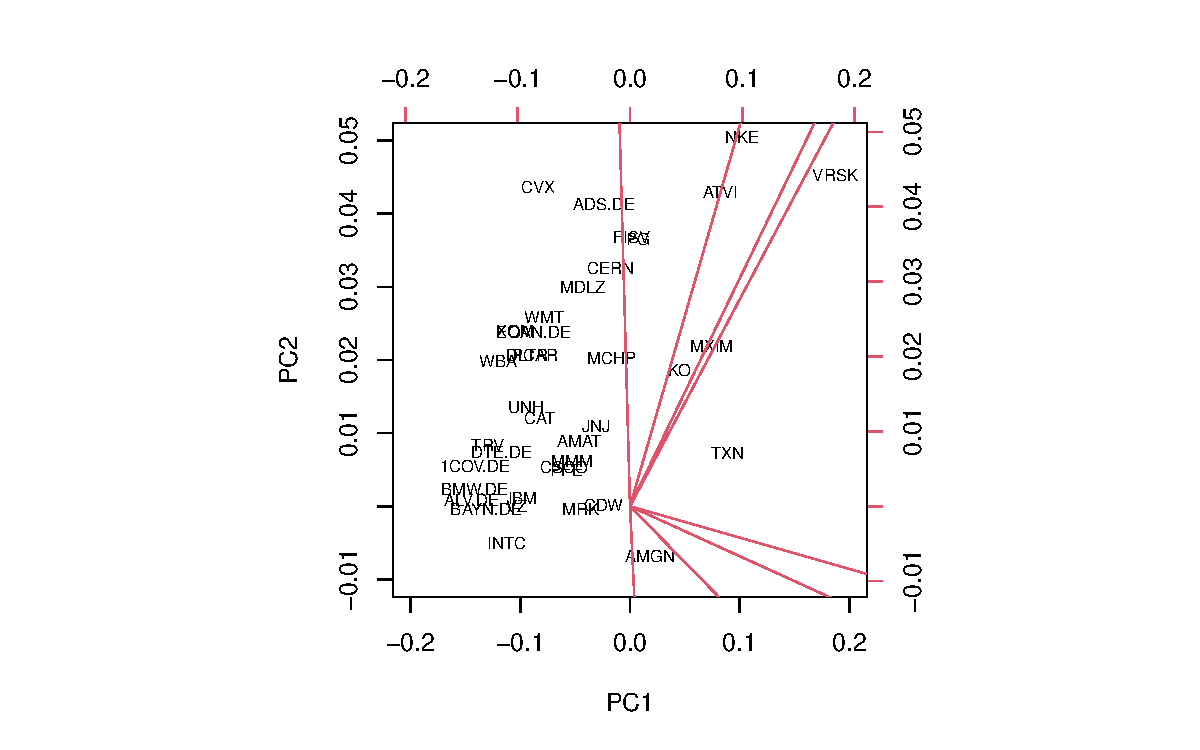
\includegraphics{ass2_files/figure-latex/value-1.pdf}

\hypertarget{value-analysisall}{%
\subsection{Value analysis(All)}\label{value-analysisall}}

\begin{verbatim}
## Importance of components:
##                           PC1    PC2    PC3    PC4     PC5     PC6     PC7
## Standard deviation     2.0937 1.4300 1.0553 0.9845 0.54966 0.31005 0.28822
## Proportion of Variance 0.4871 0.2272 0.1237 0.1077 0.03357 0.01068 0.00923
## Cumulative Proportion  0.4871 0.7143 0.8380 0.9457 0.97927 0.98996 0.99919
##                            PC8     PC9
## Standard deviation     0.08486 0.01127
## Proportion of Variance 0.00080 0.00001
## Cumulative Proportion  0.99999 1.00000
\end{verbatim}

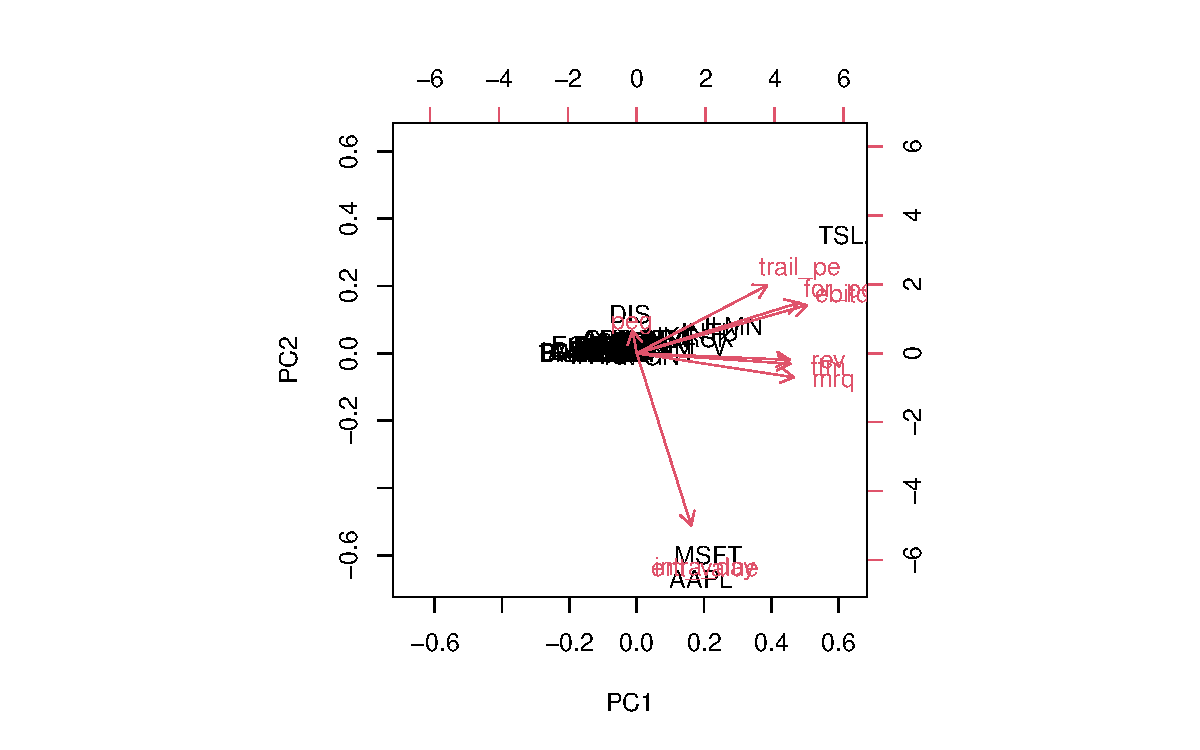
\includegraphics{ass2_files/figure-latex/unnamed-chunk-4-1.pdf} 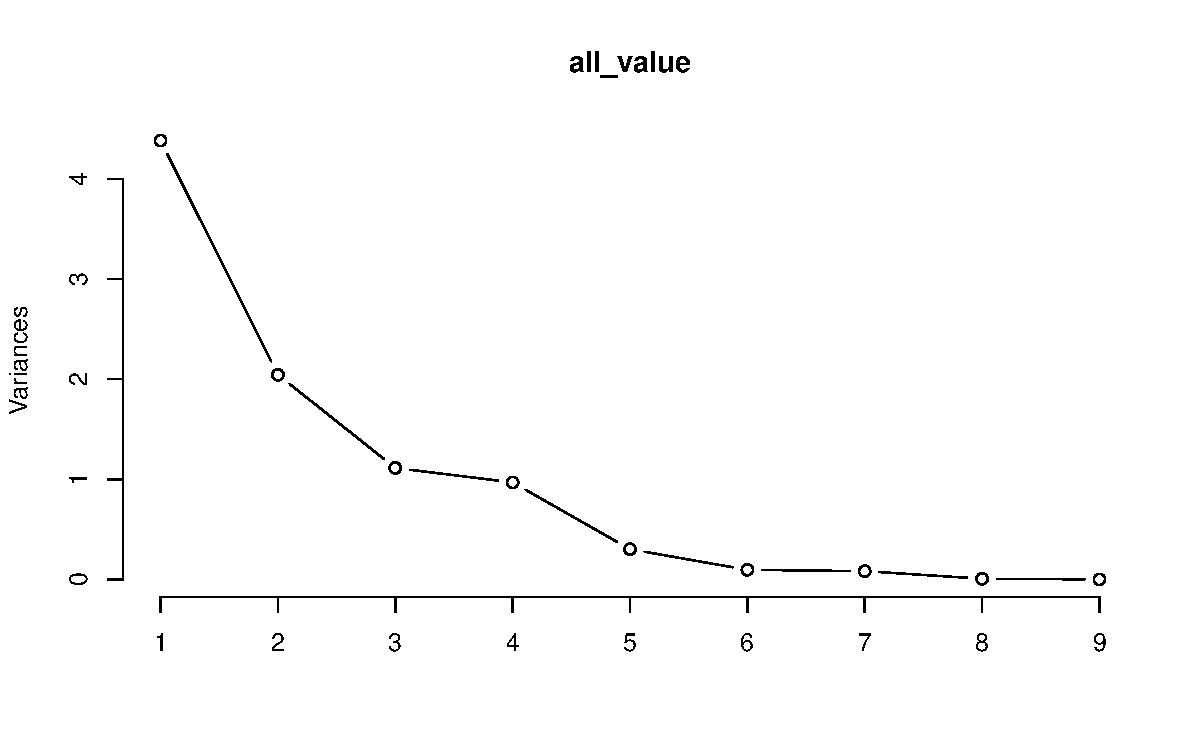
\includegraphics{ass2_files/figure-latex/unnamed-chunk-4-2.pdf}

\hypertarget{risk}{%
\subsection{Risk}\label{risk}}

\printbibliography[title=Introduction]

\end{document}

